%
%
%\begin{frame}[ctb!]
%  \frametitle{Degradation Rate Model Base Case I}
%\begin{figure}[ht]
%\centering
%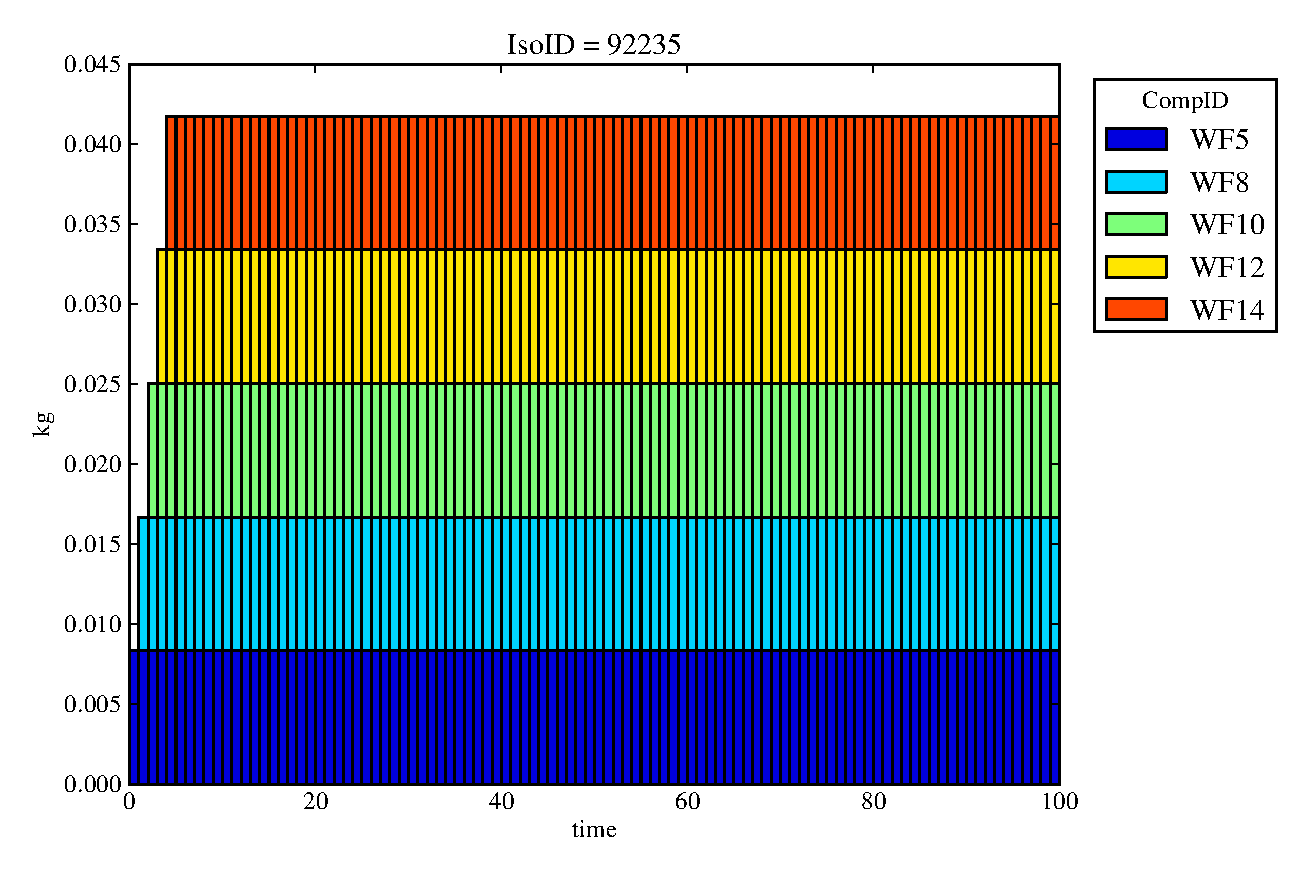
\includegraphics[width=0.8\textwidth]{./images/drI.eps}
%\caption[$^{235}U$ residence. Degradation Rate WF No Release.]{
%For Case DRI, in which total containment in the waste form is assumed ($F_{d,wf}=0$), 
%$^{235}U$ takes up permanent residence in the waste form component.
%}
%\label{fig:drIall}
%\end{figure}
%\end{frame}
%
%\begin{frame}
%  \frametitle{Degradation Rate Model Base Case I}
%  \begin{figure}
%
%\begin{minipage}[b]{0.45\linewidth}
%
%  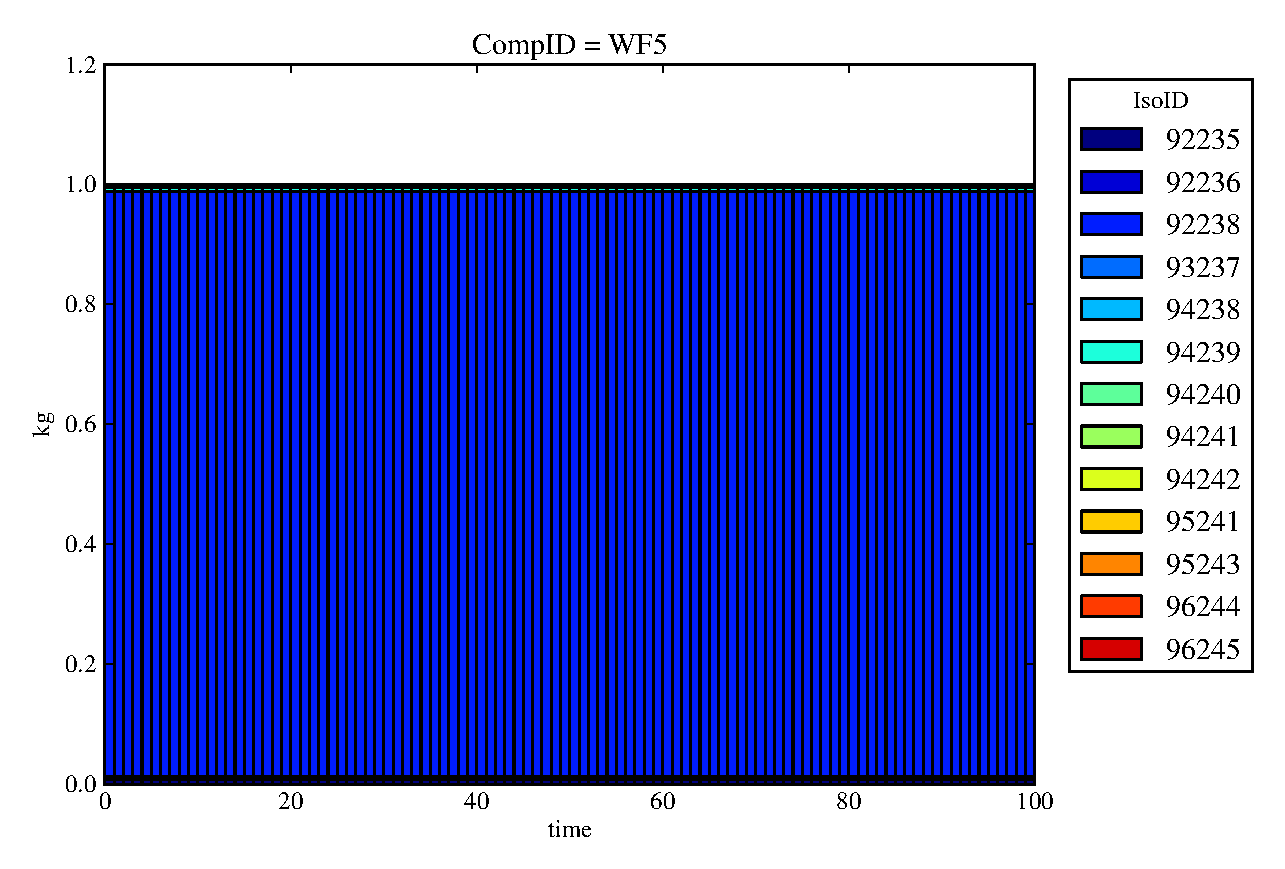
\includegraphics[width=0.8\textwidth]{./images/drI1.eps}
%  \caption[DRI WF Contaminants.]{
%    WF 5 ($F_d = 0$) never releases material.
%    }
%  \label{fig:drIwf5}
%  
%  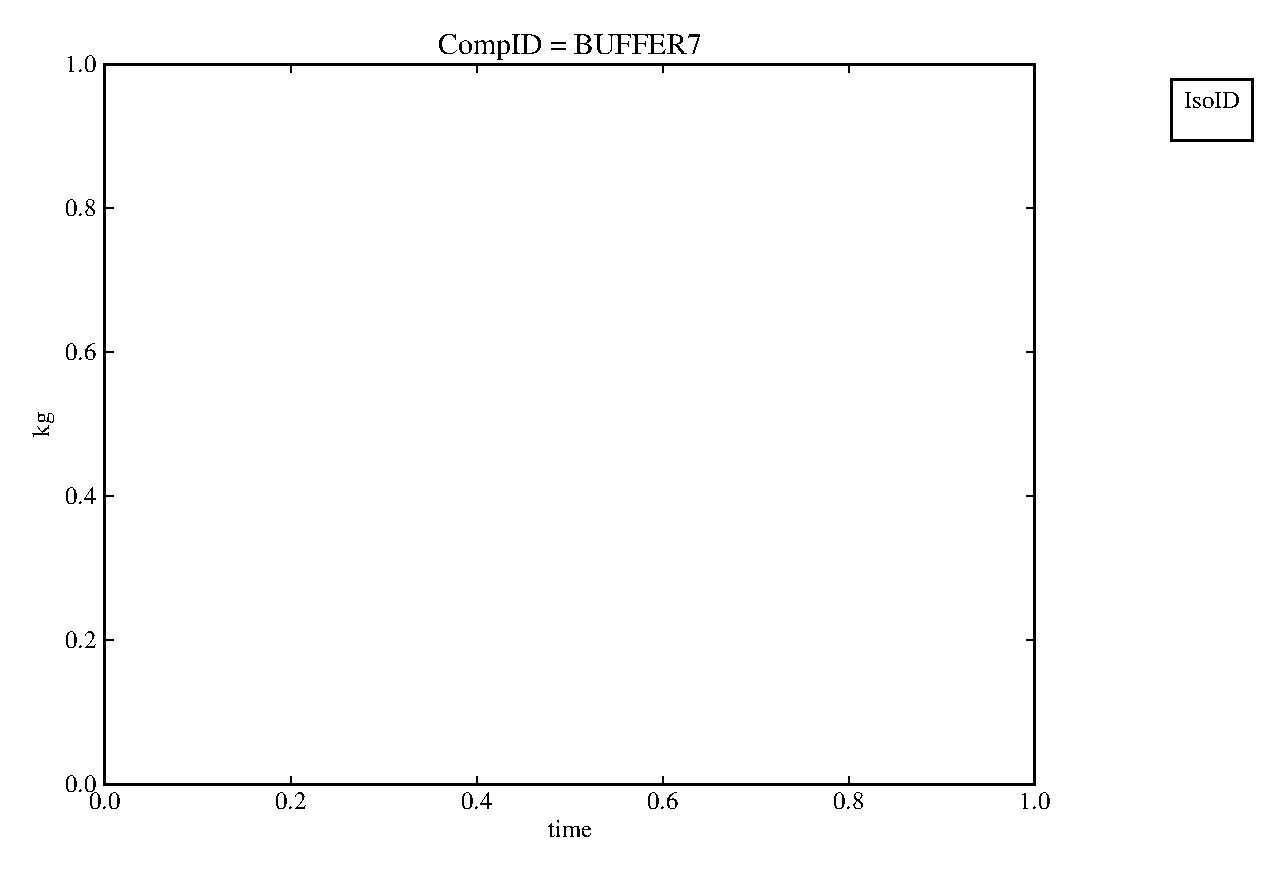
\includegraphics[width=0.8\textwidth]{./images/drI3.eps}
%  \caption[Case DRI Buffer Contaminants]{
%    The Buffer, component 7 ($F_d = 0.1$), never receives material.
%    }
%  \label{fig:drIbuff}
%
%\end{minipage}
%\hspace{0.05\linewidth}
%\begin{minipage}[b]{0.45\linewidth}
%  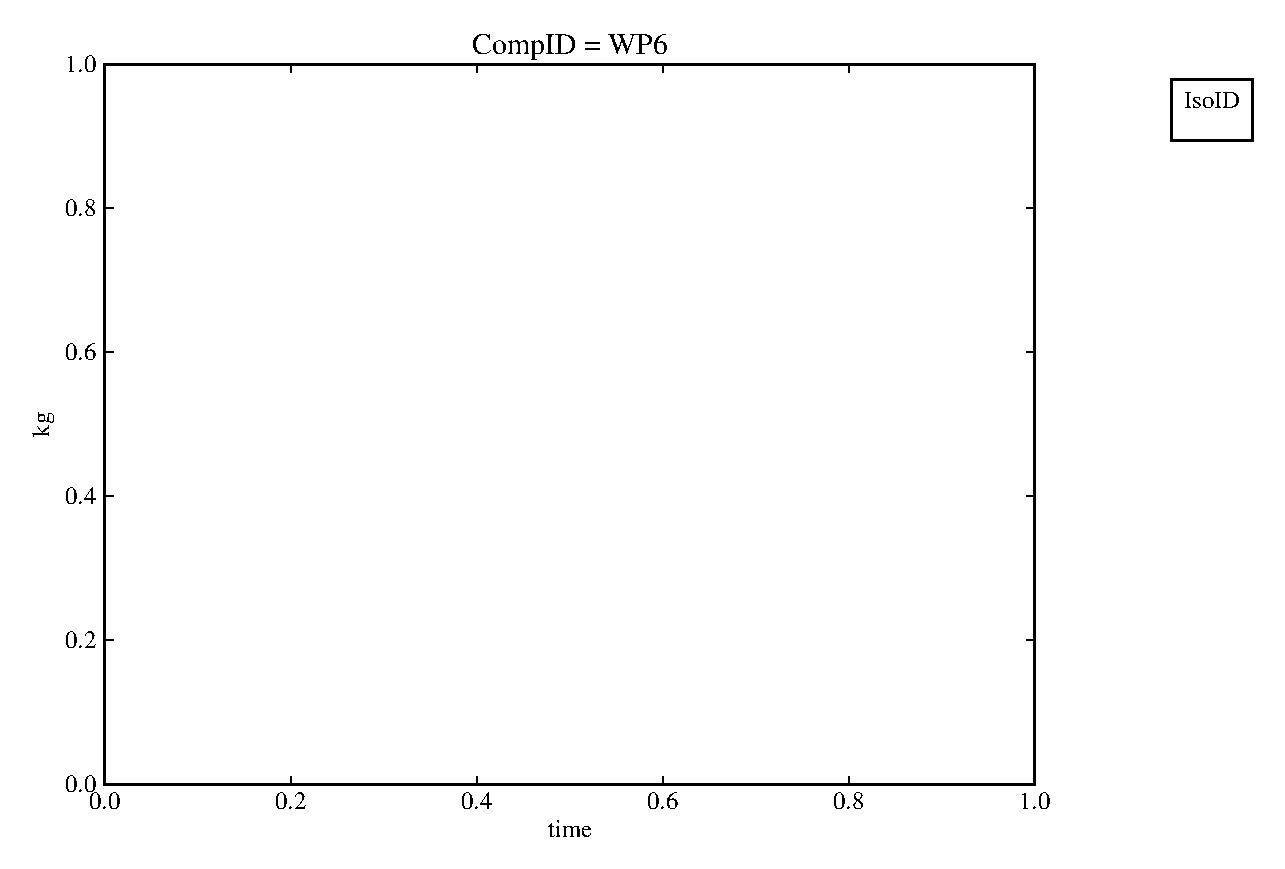
\includegraphics[width=0.8\textwidth]{./images/drI2.eps}
%  \caption[Case DRI WP Contaminants.]{ 
%    WP 6 ($F_d = 0.1$), never receives material.
%    }
%  \label{fig:drIwp6}
%
%  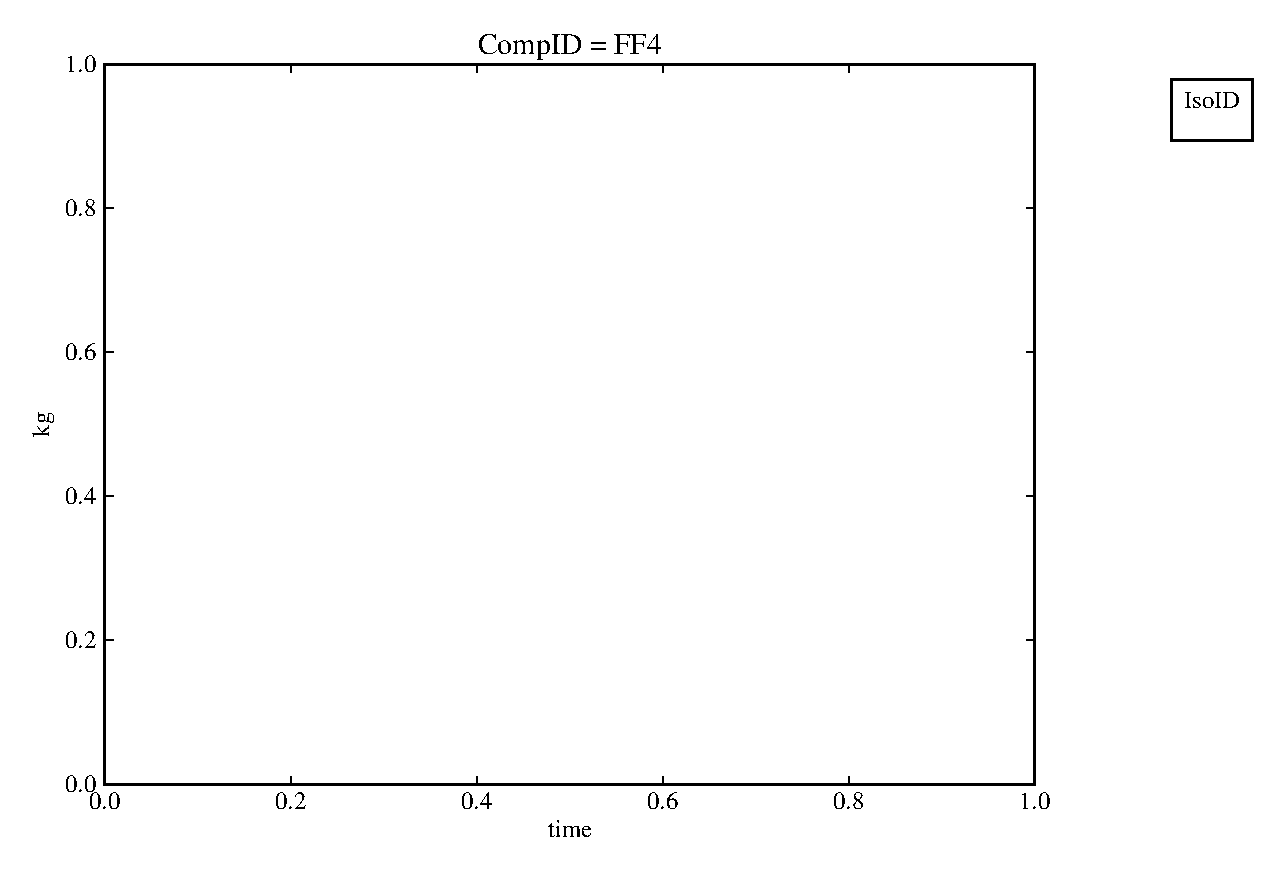
\includegraphics[width=0.8\textwidth]{./images/drI0.eps}
%  \caption[Case DRI Far Field Contaminants.]{ 
%    Far Field 4 ($F_d = 0.1$) never receives material.
%    }
%  \label{fig:drIff0}
%
%  \end{minipage}
%\end{figure}
%\end{frame}
%
%
%
%\begin{frame}[ctb!]
%  \frametitle{Degradation Rate Model Base Case II}
%\begin{figure}[ht]
%\centering
%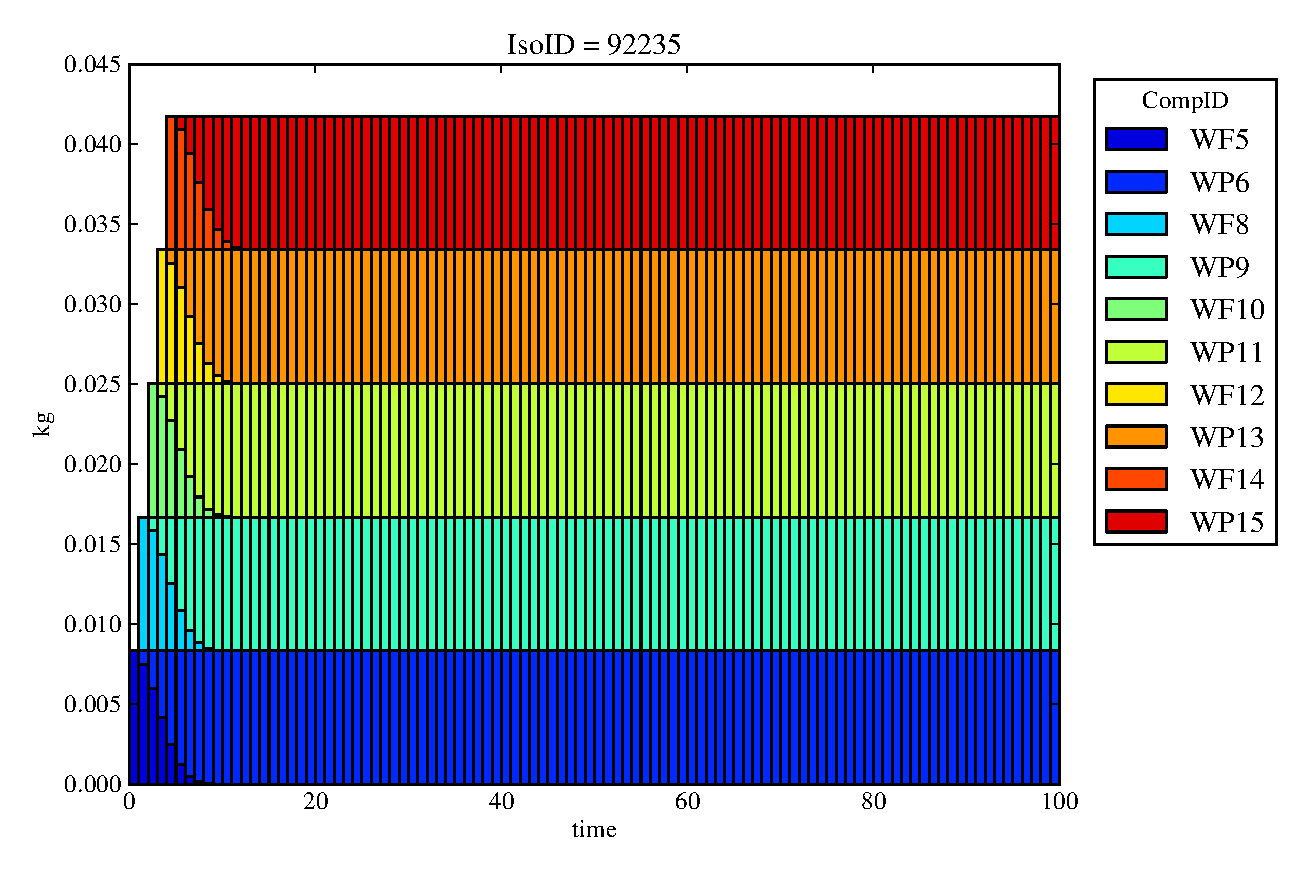
\includegraphics[width=0.8\textwidth]{./images/drII.eps}
%\caption[$^{235}U$ residence. Degradation Rate WP No Release.]{
%For Case DRII, in which total containment in the waste package is assumed ($F_{d,wp}=0$), 
%$^{235}U$ travels through waste forms ($F_d = 0.1$) before 
%permanent residence in the waste package components.
%}
%\label{fig:drIIall}
%\end{figure}
%\end{frame}
%
%\begin{frame}
%  \frametitle{Degradation Rate Model Base Case II}
%  \begin{figure}
%\begin{minipage}[b]{0.45\linewidth}
%
%  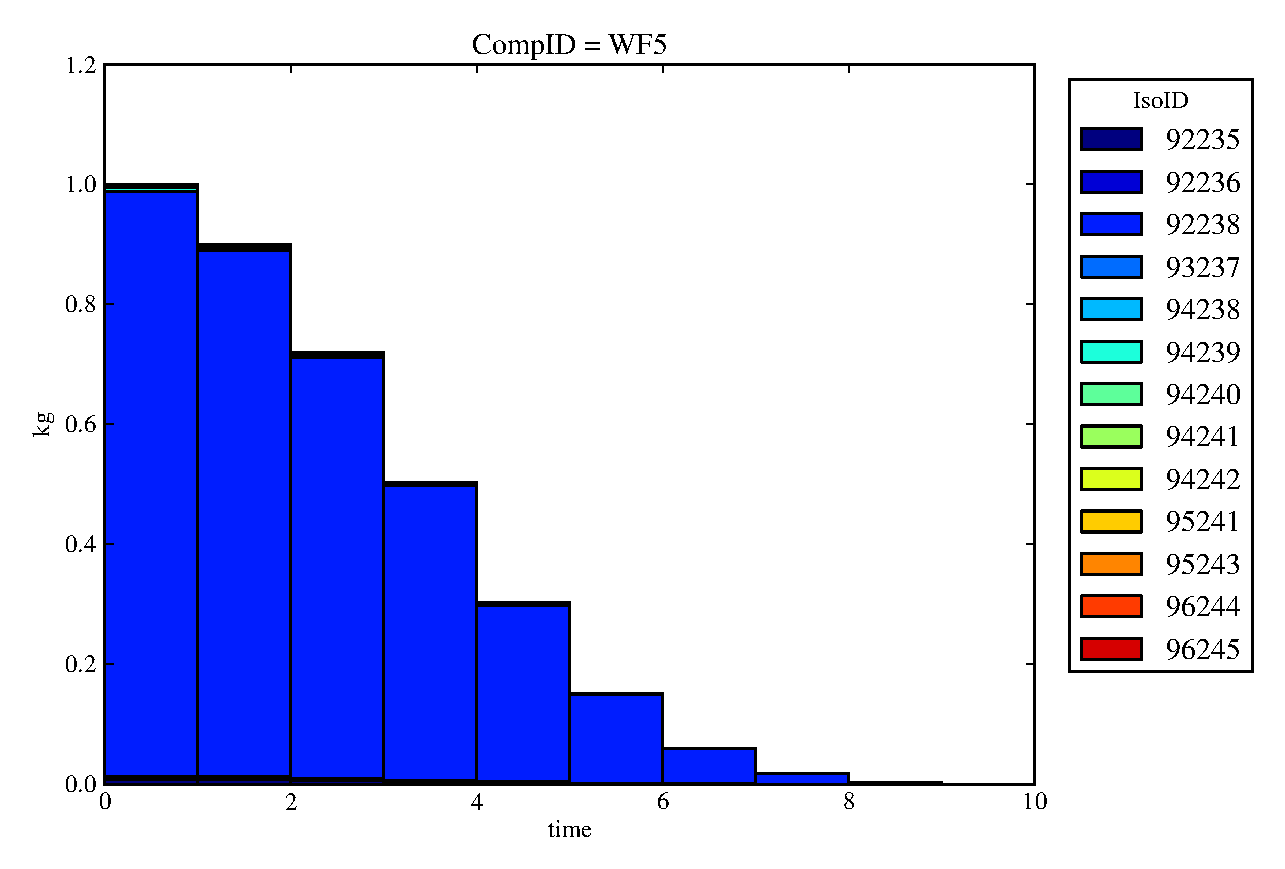
\includegraphics[width=0.8\textwidth]{./images/drII1.eps}
%  \caption[DRII WF Contaminants.]{
%    WF 5 ($F_d = 0.1$) releases material with degradation. 
%    }
%  \label{fig:drIIwf5}
%  
%  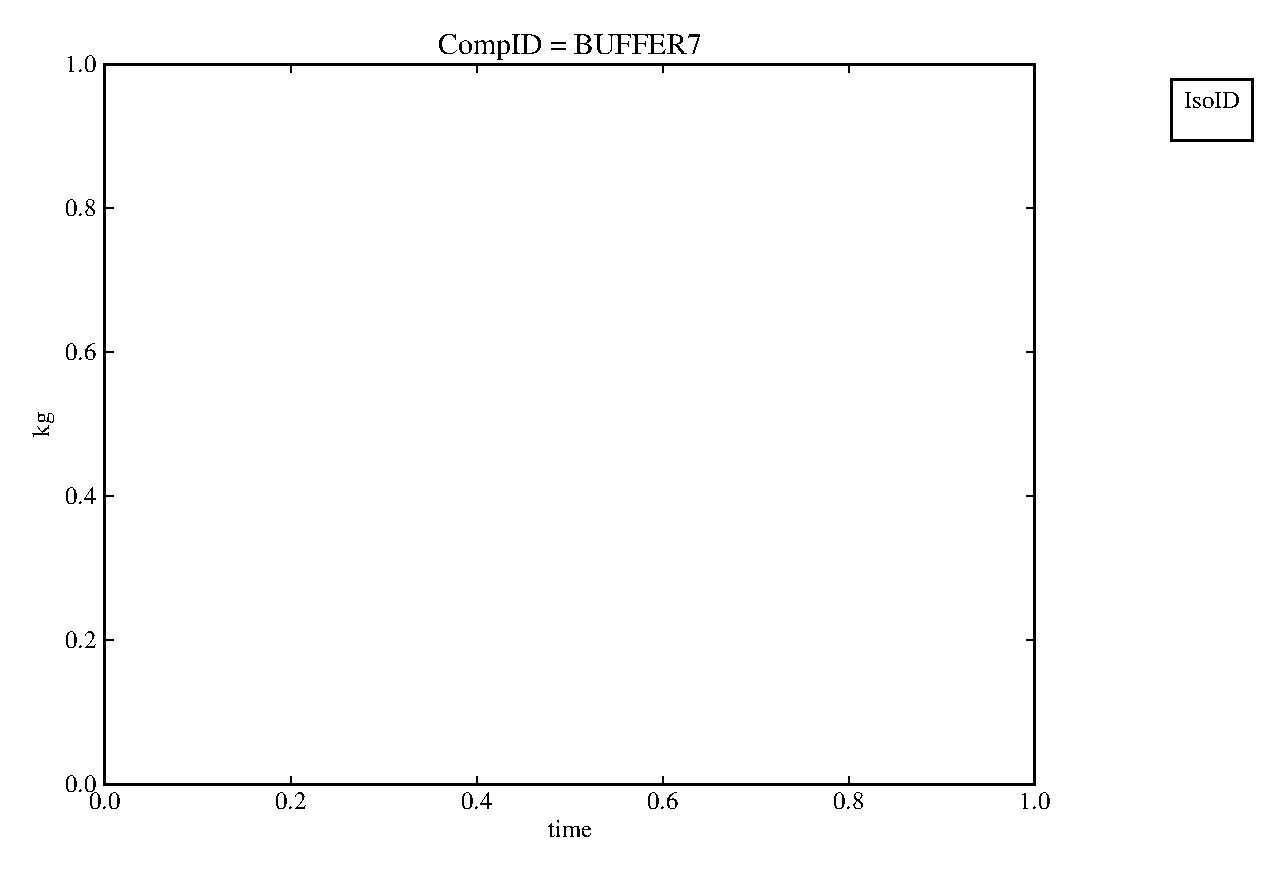
\includegraphics[width=0.8\textwidth]{./images/drII3.eps}
%  \caption[Case DRII Buffer Contaminants]{
%    The Buffer, component 7 ($F_d = 0.1$), never receives material.
%    }
%  \label{fig:drIIbuff}
%
%\end{minipage}
%\hspace{0.05\linewidth}
%\begin{minipage}[b]{0.45\linewidth}
%  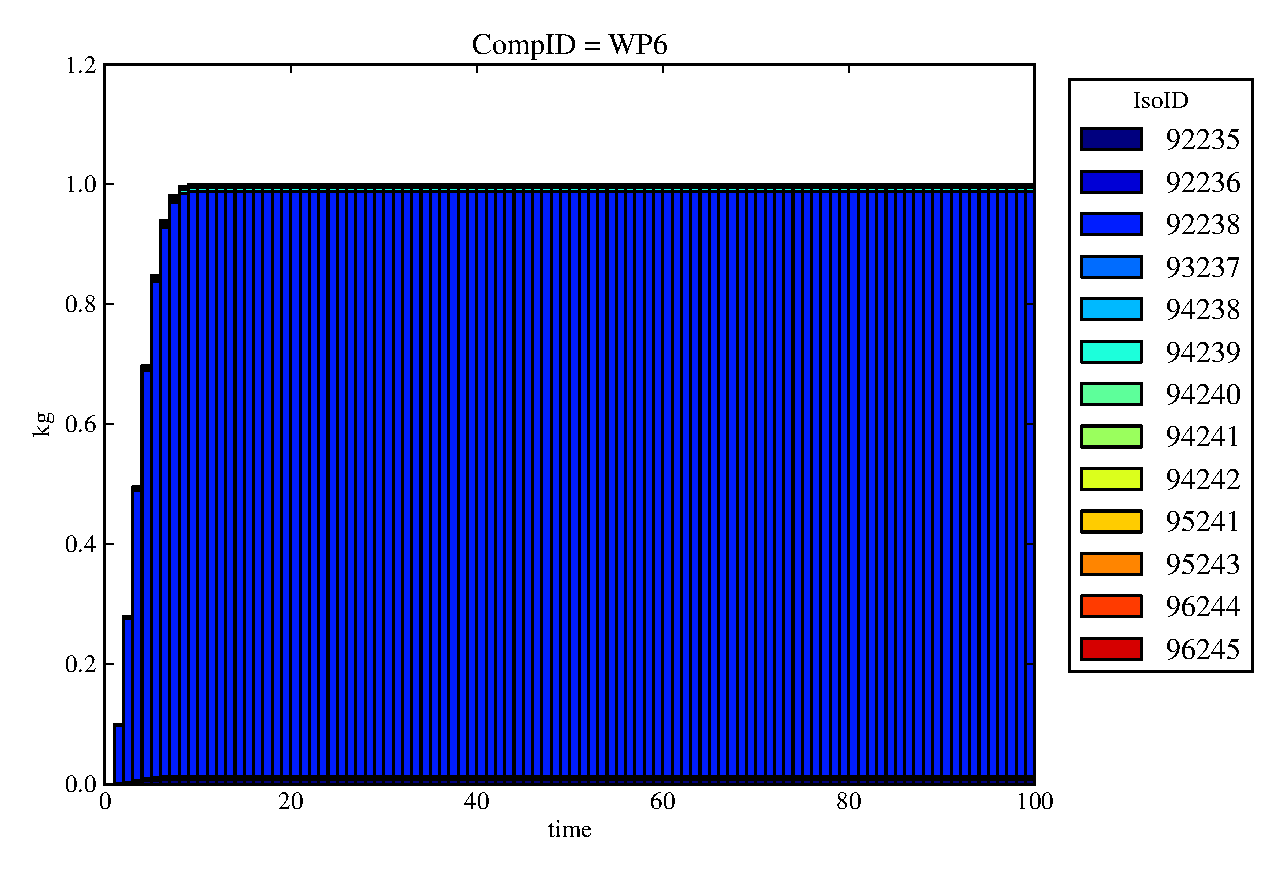
\includegraphics[width=0.8\textwidth]{./images/drII2.eps}
%  \caption[Case DRII WP Contaminants.]{ 
%    WP 6 ($F_d = 0$) acheives total containment.
%    }
%  \label{fig:drIIwp6}
%
%  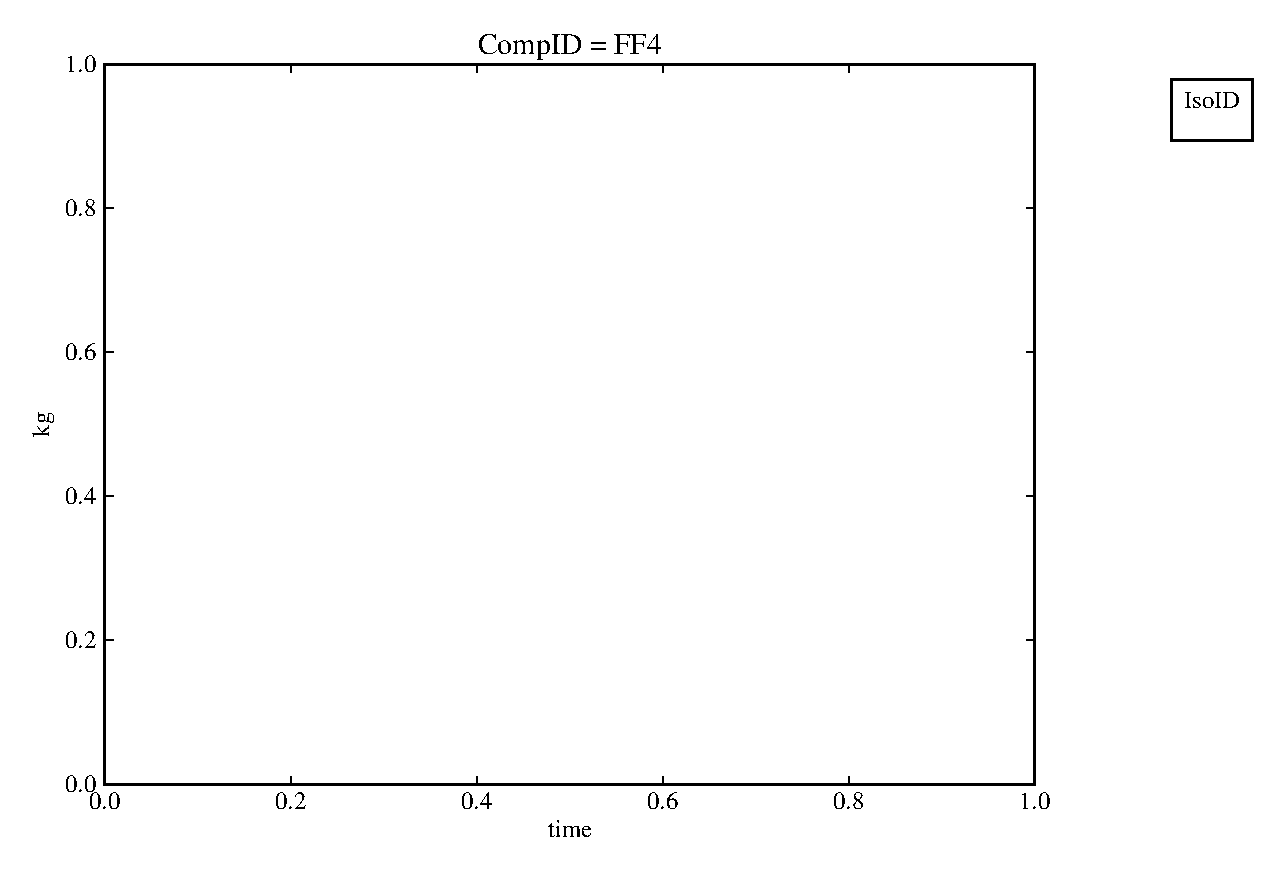
\includegraphics[width=0.8\textwidth]{./images/drII0.eps}
%  \caption[Case DRII Far Field Contaminants.]{ 
%    Far Field 4 ($F_d = 0.1$), never receives material.
%    }
%  \label{fig:drIIff0}
%
%
%  \end{minipage}
%\end{figure}
%\end{frame}
%
\begin{frame}[ctb!]
\begin{figure}[ht]
  \frametitle{Degradation Rate Model Base Case III}
\centering
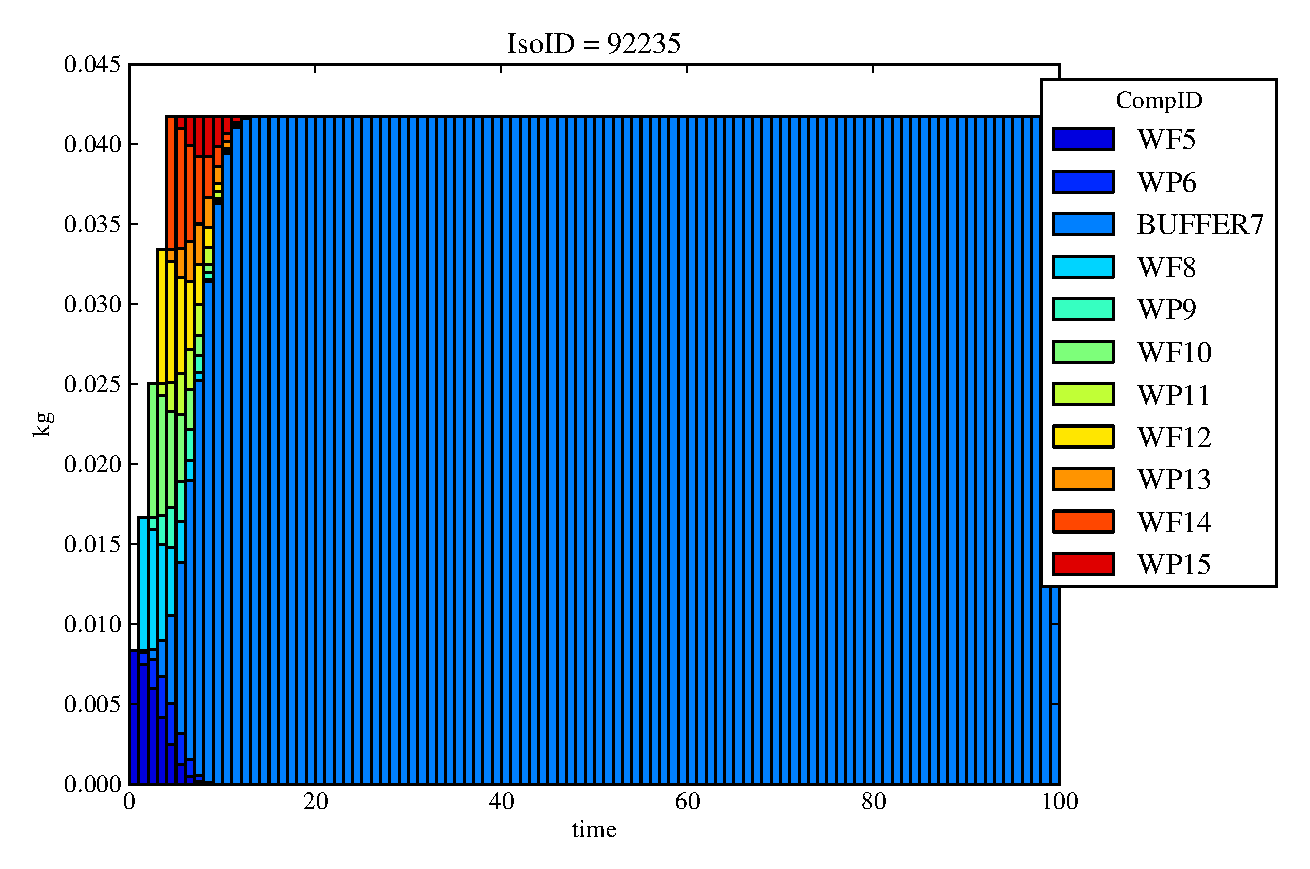
\includegraphics[width=0.8\textwidth]{./images/drIII.eps}
\caption[$^{235}U$ residence. Degradation Rate Buffer No Release.]{
For Case DRIII, in which total containment in the buffer is assumed ($F_{d,buffer}=0$), 
$^{235}U$ travels through waste forms and waste package components ($F_d = 0.1$) before 
permanent residence in the buffer component.
}
\label{fig:drIIIall}
\end{figure}
\end{frame}

\begin{frame}
  \frametitle{Degradation Rate Model Base Case III}
  \begin{figure}
\begin{minipage}[b]{0.45\linewidth}

  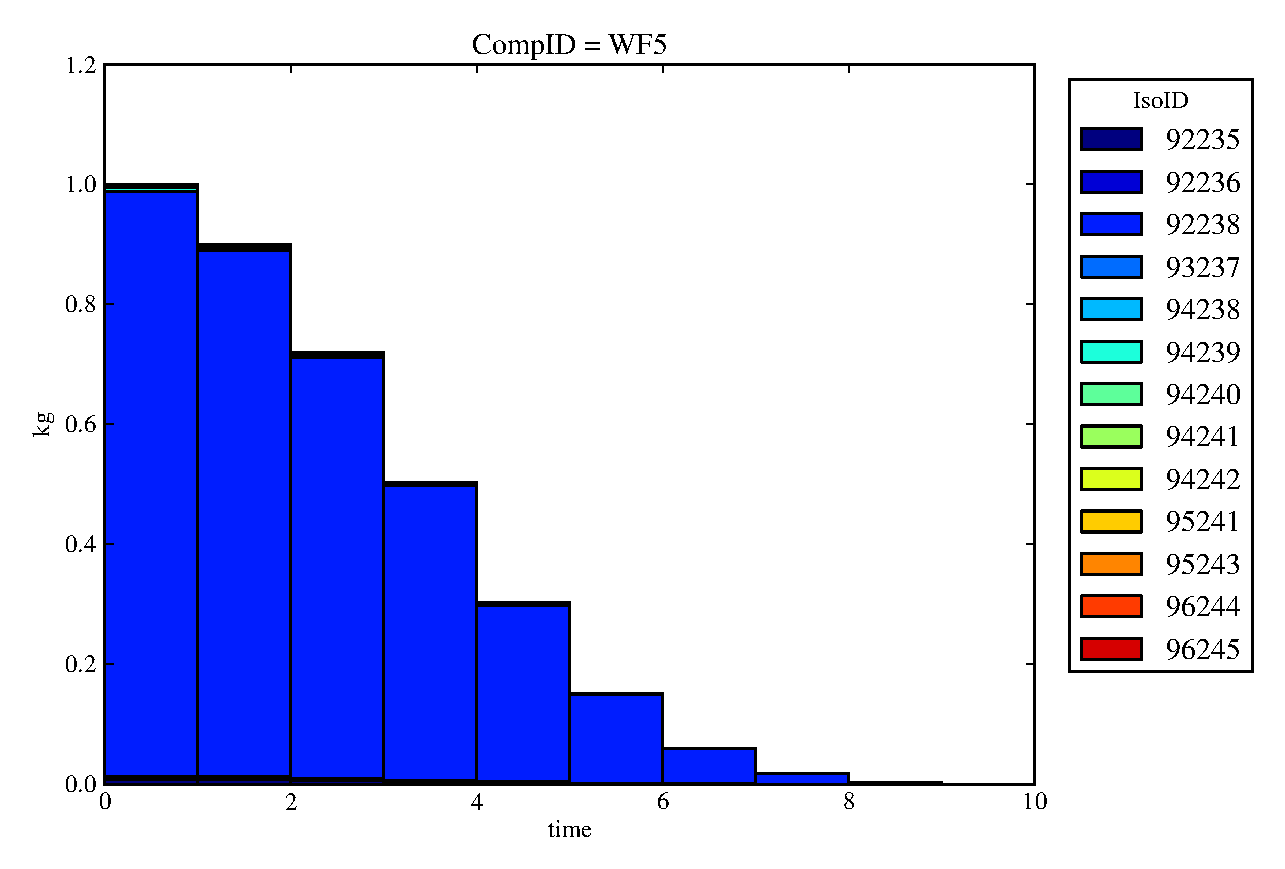
\includegraphics[width=0.8\textwidth]{./images/drIII1.eps}
  \caption[DRIII WF Contaminants.]{
    WF 5 ($F_d = 0.1$) releases material with degradation. 
    }
  \label{fig:drIIIwf5}
  
  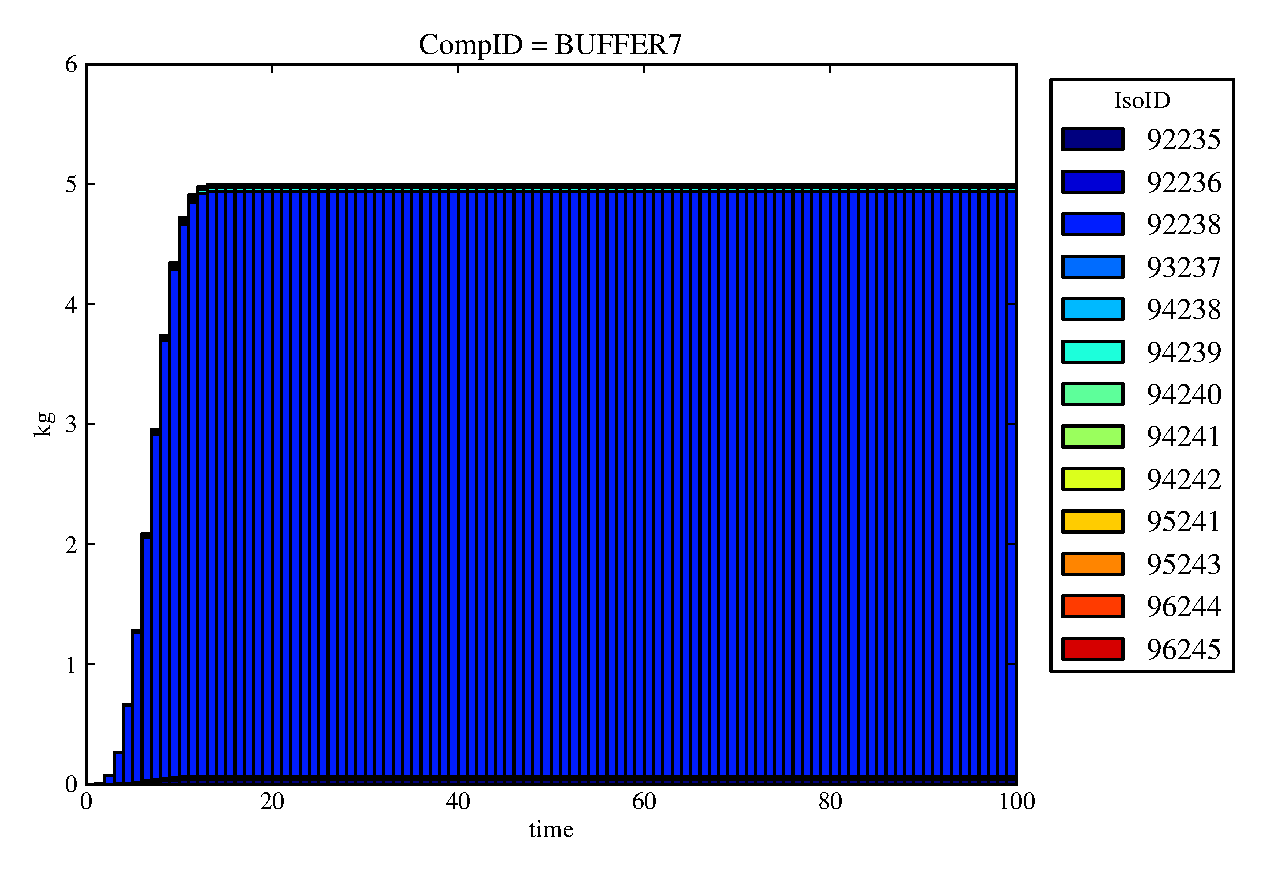
\includegraphics[width=0.8\textwidth]{./images/drIII3.eps}
  \caption[Case DRIII Buffer Contaminants]{
    Buffer 7 ($F_d=0$) acheives total containment.
    }
  \label{fig:drIIIbuff}

\end{minipage}
\hspace{0.05\linewidth}
\begin{minipage}[b]{0.45\linewidth}
  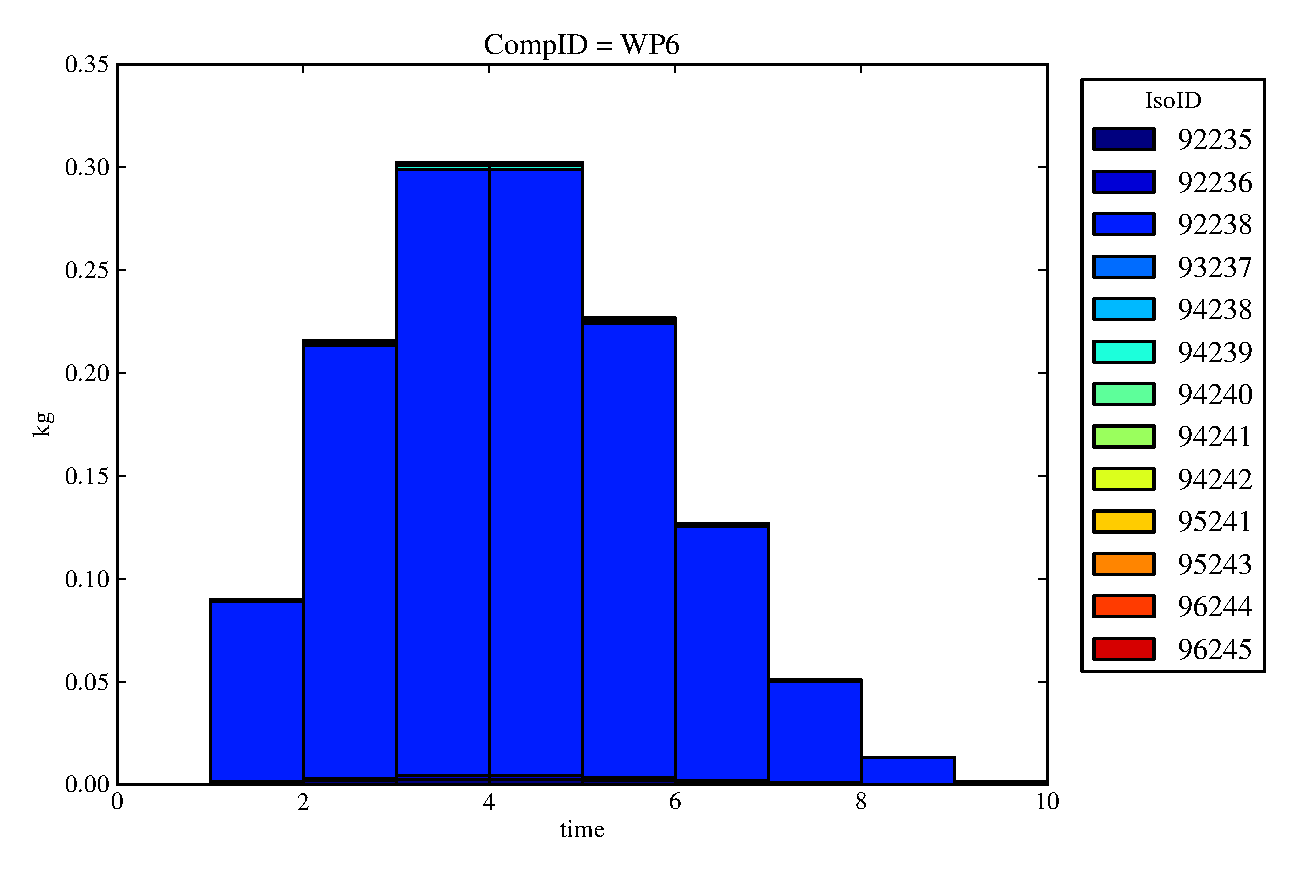
\includegraphics[width=0.8\textwidth]{./images/drIII2.eps}
  \caption[Case DRIII WP Contaminants.]{ 
    WP 6 ($F_d = 0.1$) receives and releases material. 
    }
  \label{fig:drIIIwp6}

  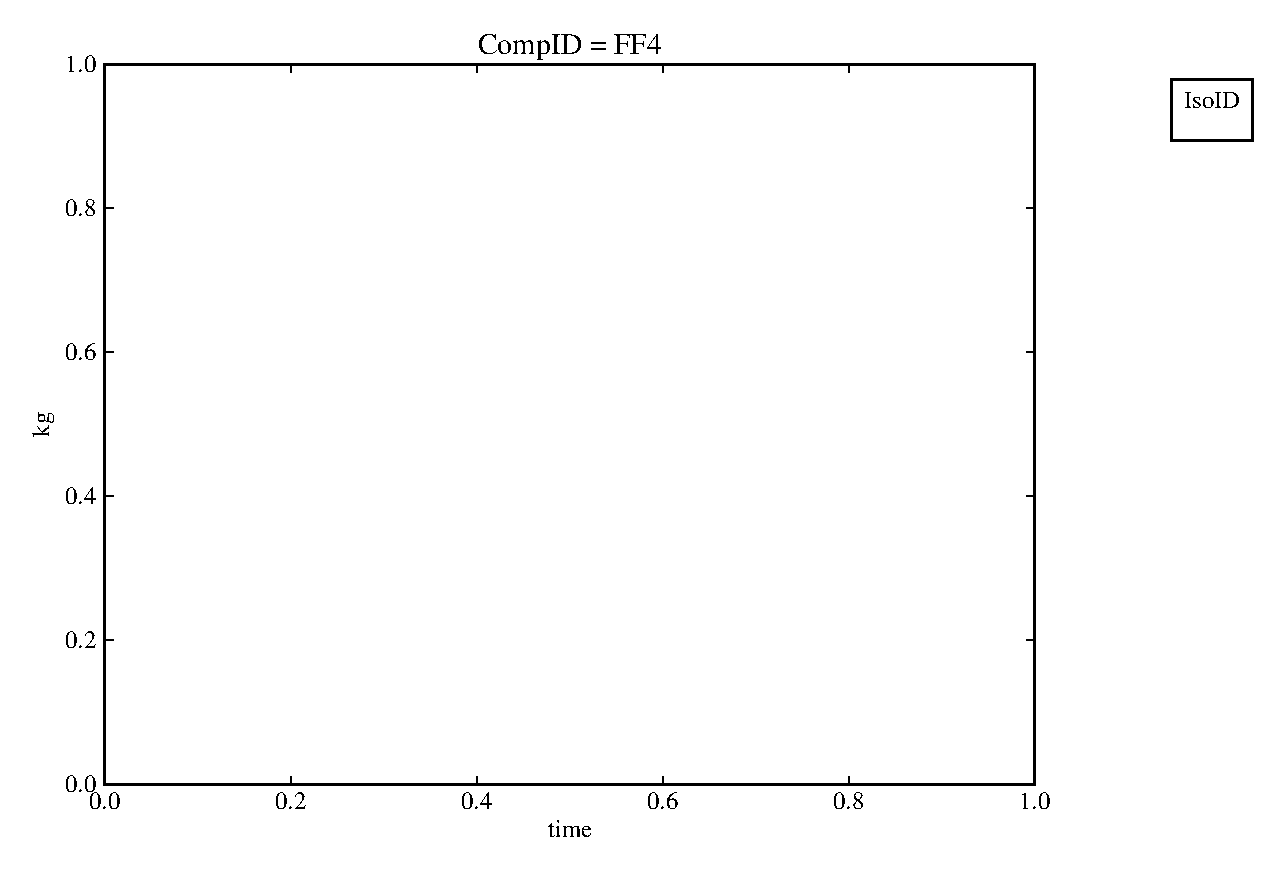
\includegraphics[width=0.8\textwidth]{./images/drIII0.eps}
  \caption[Case DRIII WP Contaminants.]{ 
    Far Field 4 ($F_d = 0.1$), never receives material.
    }
  \label{fig:drIIIff0}


  \end{minipage}
\end{figure}
\end{frame}


\begin{frame}[ctb!]
  \frametitle{Degradation Rate Model Base Case IV}

\begin{figure}[ht]
\centering
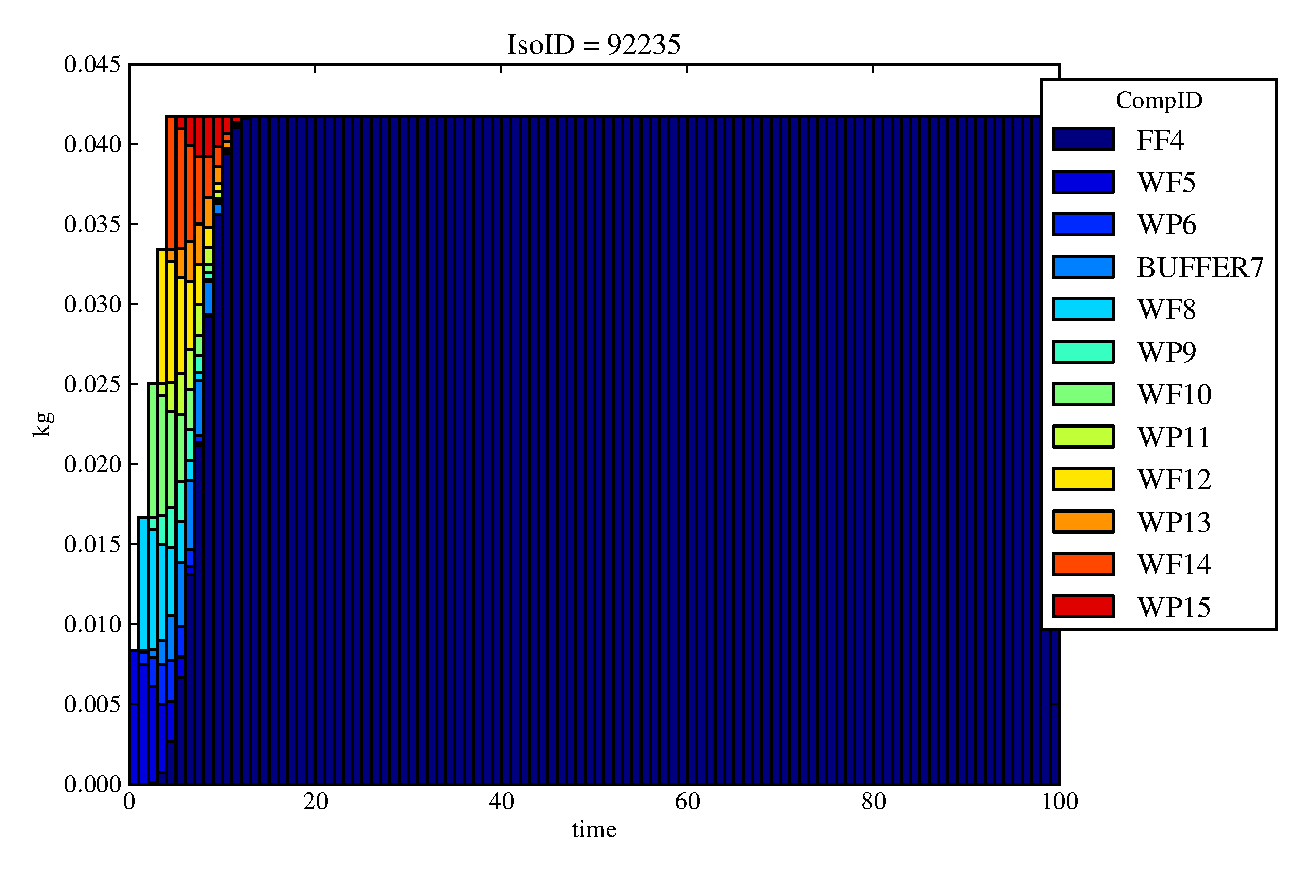
\includegraphics[width=0.8\textwidth]{./images/drIV.eps}
\caption[$^{235}U$ residence. Degradation Rate Buffer No Release.]{
For DRIV case in which total containment in the far field is assumed ($F_{d,ff}=0$), 
$^{235}U$ travels through interior components ($F_d = 0.1$) before 
permanent residence in the far field component.
}
\label{fig:drIVall}
\end{figure}
\end{frame}

\begin{frame}
  \frametitle{Degradation Rate Model Base Case IV}
  \begin{figure}
\begin{minipage}[b]{0.45\linewidth}

  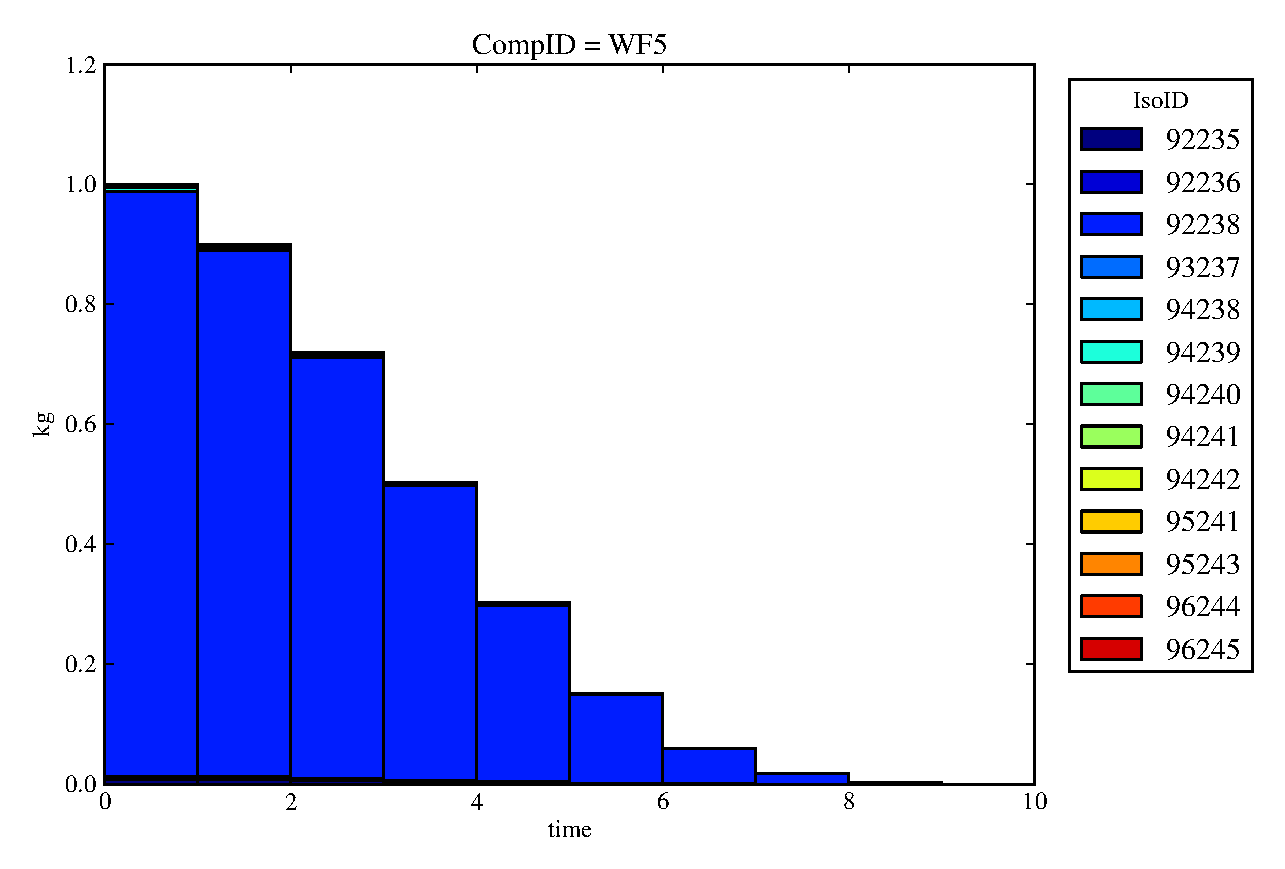
\includegraphics[width=0.8\textwidth]{./images/drIV1.eps}
  \caption[DRIV WF Contaminants.]{
    WF 5 ($F_d = 0.1$) releases material with degradation. 
    }
  \label{fig:drIVwf5}
  
  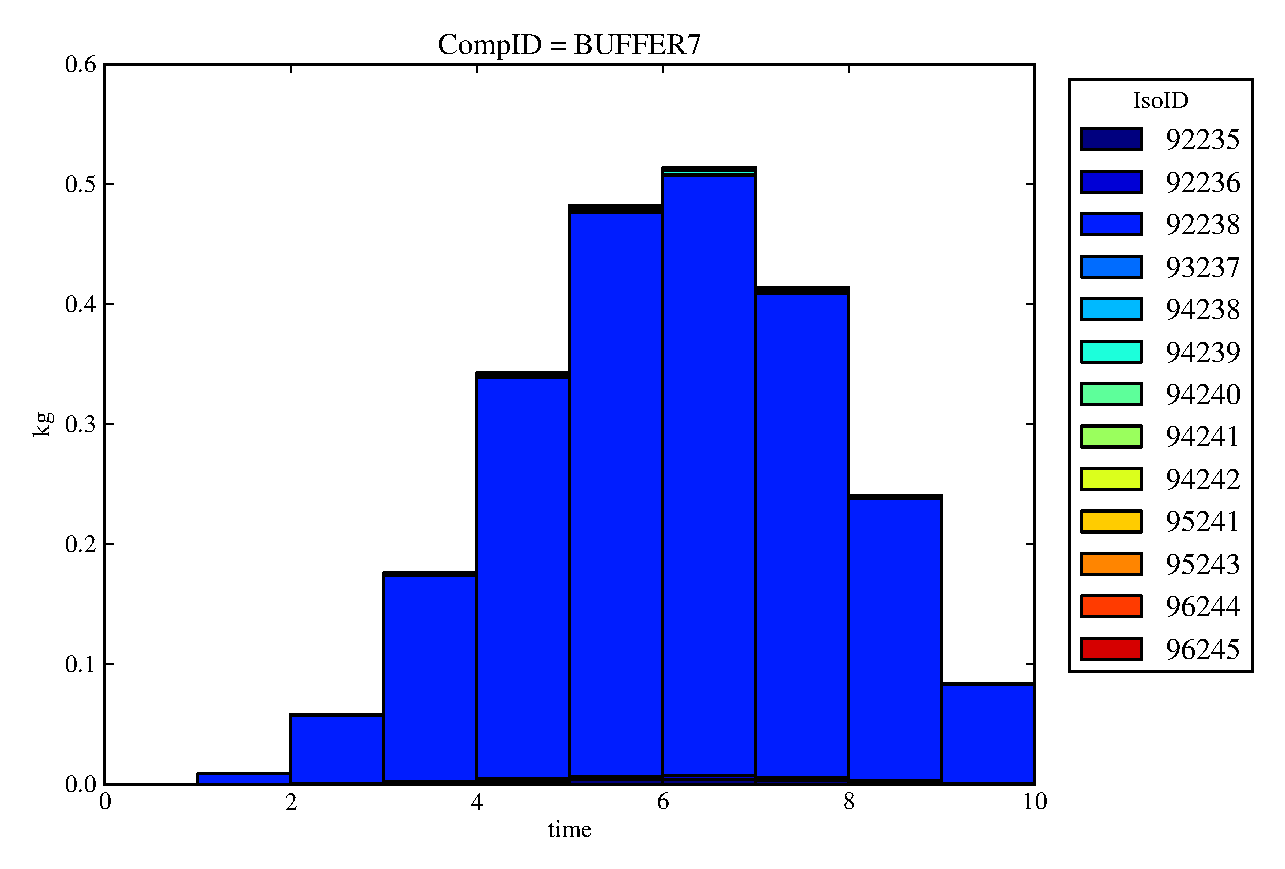
\includegraphics[width=0.8\textwidth]{./images/drIV3.eps}
  \caption[Case DRIV Buffer Contaminants]{
    The Buffer, component 7 ($F_d=0.0$), receives and then releases material.
    }
  \label{fig:drIVbuff}

\end{minipage}
\hspace{0.05\linewidth}
\begin{minipage}[b]{0.45\linewidth}
  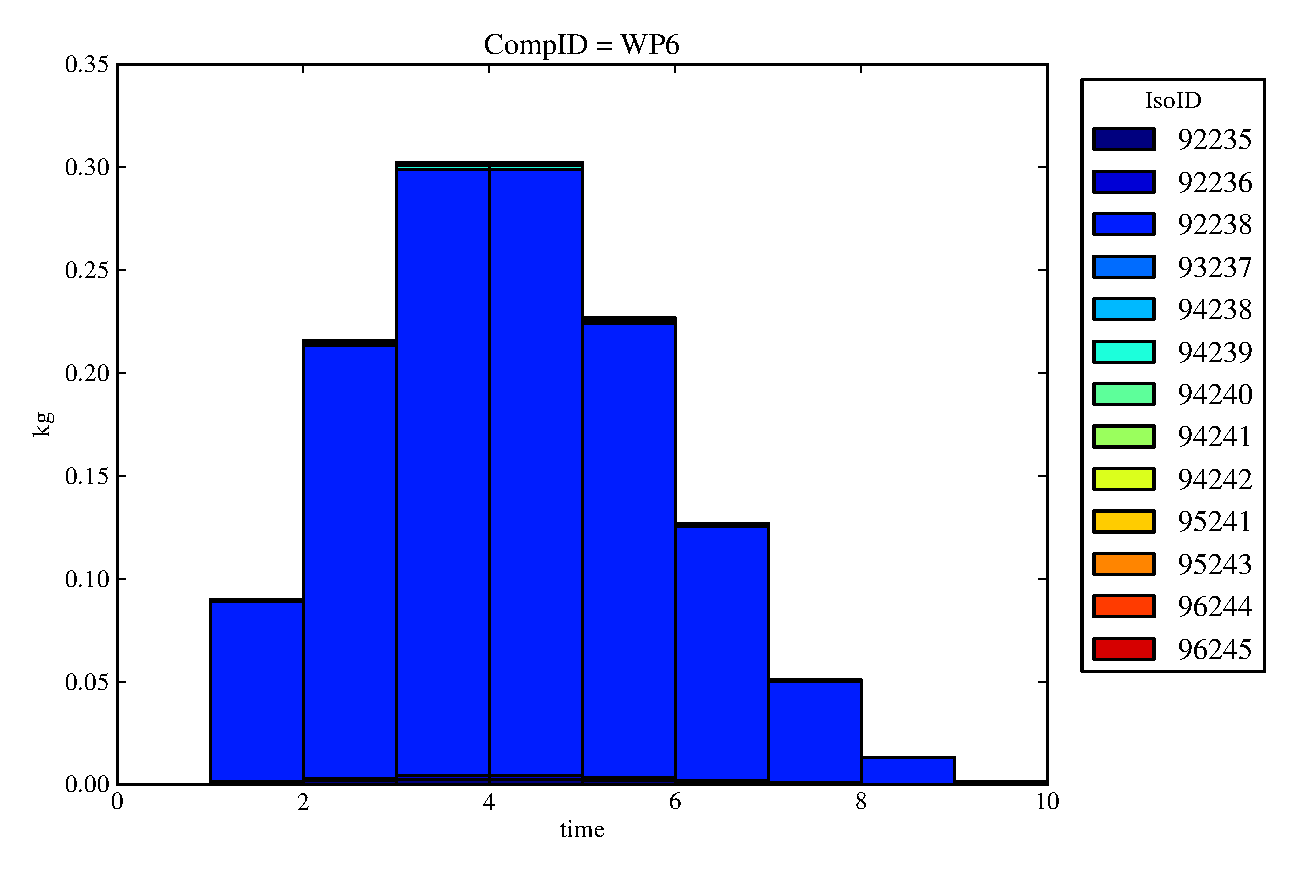
\includegraphics[width=0.8\textwidth]{./images/drIV2.eps}
  \caption[Case DRIV WP Contaminants.]{ 
    WP 6 ($F_d = 0.1$) receives and releases material. 
    }
  \label{fig:drIVwp6}

  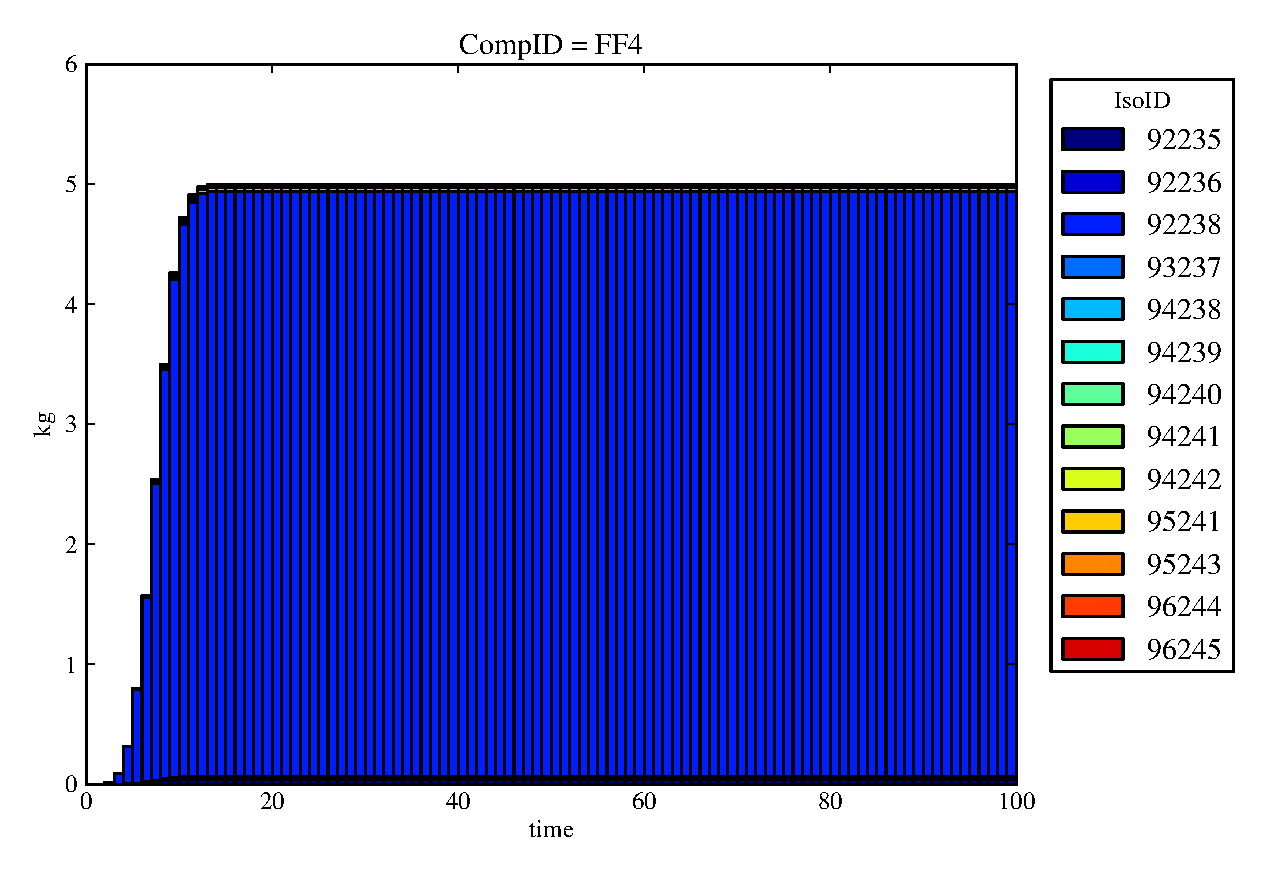
\includegraphics[width=0.8\textwidth]{./images/drIV0.eps}
  \caption[Case DRIV WP Contaminants.]{ 
    Far Field 4 ($F_d = 0.0$), acheives total containment.
    }
  \label{fig:drIVff0}


  \end{minipage}
\end{figure}
\end{frame}
